In the search for SUSY in the compressed spectrum scenario presented in
\cref{cha:monojet-signature} of this thesis, the HLT\_xe70 trigger is used, it
receives an L1 accept that selects events with a missing energy (see
\cref{sec:miss-transv-energy}) greater than 50~GeV computed at the L1 trigger.
No muons are used in the reconstruction of the missing energy at the trigger
level. The events that survive L1 are then passed to the \gls{hlt} level, where
events with a missing energy (calculated from cell energy information) greater
than 70~GeV are selected.

\cref{fig:lumi_summary} shows the delivered luminosity as a function of the
average number of interactions per bunch crossing $\langle \mu \rangle$ during
the 2015 and 2016 data taking periods. Due to the increasing luminosity and
pile-up (see \cref{sec:primary-vertex}), in the search for large extra
dimensions in the \gls{add} model scenario presented in
\ref{cha:2016-monoj-analys} of this thesis the trigger had to be modified. A
combination of four different triggers is used, they all pass the level one
trigger selection if the event have a missing energy of more than 50~GeV at L1,
again no muon information is used in the missing energy reconstruction at this
level. For the \gls{hlt} the missing energy threshold is increased in steps of
10~GeV from 80~GeV up to 110~GeV for the four different triggers. The
information on the missing energy takes advantage of the
\gls{mht}~\cite{MHTAlgorithm} algorithm or the \gls{lcw}~\cite{LCWCalibration}
calibration scheme depending on the trigger used. In the \gls{mht} algorithm the
missing energy is calculated as the negative vector sum of the transverse
momentum ($- \sum \pt^\mathrm{\, jets} \equiv - H_\mathrm{\, T}$) of all the
jets reconstructed with the $\antikt$ jet finding algorithm (see
\cref{sec:anti-k_t}) from topoclusters (see \cref{sec:topocluster}). The
\gls{lcw} calibration scheme uses the shape of the cluster and the energy
density to classify the topocluster energy deposits as electromagnetic or
hadronic improving the resolution of the missing energy trigger.

\cref{tab:trigger_periods} summarizes the different trigger combination for the
2016 dataset used in the analysis. The increase with time of the maximum
instantaneous luminosity $\mathcal{L}^{max}$ forced the use of a higher missing
energy threshold in the trigger. \cref{fig:trigger_efficiency} shows the trigger
efficiency for the four different data taking periods in the 2016 analysis as a
function of the missing energy as evaluated offline (i.e.\@ the same variable
used in the analyses) estimated using $\wmunuplusjets$ events. It can be seen
that the trigger is fully efficient from approximately 200~GeV. The monojet
analyses presented in \cref{cha:monojet-signature,cha:2016-monoj-analys} require
a missing transverse energy of at least 250~GeV and are therefore not affected
by the loss of efficiency below 200~GeV.
% receive an L1 accept for events with more than 50~GeV of missing energy, with no
% muon information for the missing energy reconstruction at this level.
% HLT\_xe80\_tc\_lcw\_L1XE50, HLT\_xe90\_mht\_L1XE50,
% HLT\_xe100\_mht\_L1XE50 and HLT\_xe110\_mht\_L1XE50. The
% HLT\_xe80\_tc\_lcw\_L1XE50 at L1 level selects events with a missing energy of
% more than 50~GeV while at the \gls{hlt} level it uses the \gls{lcw} to calibrate
% the missing energy whose information is taken from the energy deposited in the
% topocluster (tc) (see \cref{sec:topocluster}). The \gls{lcw} uses the
\begin{table}[!ht]
  \centering
    \resizebox{\linewidth}{!}{\begin{tabular}{lcc}
    \toprule
    \multicolumn{3}{c}{Trigger Used in the 2016 Analysis} \\
    \midrule \midrule
    Run Range & Trigger & $\mathcal{L}^{max} (10^{30} cm^{-2}s^{-1})$ \\
    \midrule
    296939-302393 & HLT\_xe90\_mht\_L1XE50 or HLT\_xe80\_tc\_lcw\_L1XE50 & 8761 \\
    302737-302872 & HLT\_xe90\_mht\_L1XE50 & 9854 \\
    302919-304008 & HLT\_xe100\_mht\_L1XE50 or HLT\_xe110\_mht\_L1XE50 & 10261 \\
    304128-310216 & HLT\_xe110\_mht\_L1XE50 & 13716 \\
    \bottomrule
  \end{tabular}}
\caption{The table reports the trigger used in the 2016 data taking. The maximum
  instantaneous luminosity $\mathcal{L}^{max} (10^{30} cm^{-2}s^{-1})$ is also
  reported. The constant increasing of $\mathcal{L}^{max}$ justifies the choice
  of higher $\met$ thresholds for the trigger.}
  \label{tab:trigger_periods}
\end{table}
% \begin{table}[!ht]
%   \centering
%   \begin{tabular}{lcc}
%     \toprule
%     \multicolumn{3}{c}{Trigger Used In The 2016 Data Taking} \\
%     \midrule \midrule
%     Run Range & Trigger & $\langle \mu \rangle$ \\
%     \midrule
%     296939-302393 & HLT\_xe90\_mht\_L1XE50 or HLT\_xe80\_tc\_lcw\_L1XE50 & 33.1 \\
%     302737-302872 & HLT\_xe90\_mht\_L1XE50 & 34 \\
%     302919-304008 & HLT\_xe100\_mht\_L1XE50 or HLT\_xe110\_mht\_L1XE50 & 35.4 \\
%     304128-310216 & HLT\_xe110\_mht\_L1XE50 & 51.1 \\
%     \bottomrule
%   \end{tabular}
%   \caption{The table reports the trigger used in the 2016 data taking. The
%     average number of interactions per bunch crossing, $\langle \mu \rangle$, is
%   also reported. The constant increasing of $\langle \mu \rangle$ justifies the
%   choice of higher $\met$ thresholds for the trigger.}
%   \label{tab:trigger_periods}
% \end{table}
\begin{figure}[!ht]
  \centering
    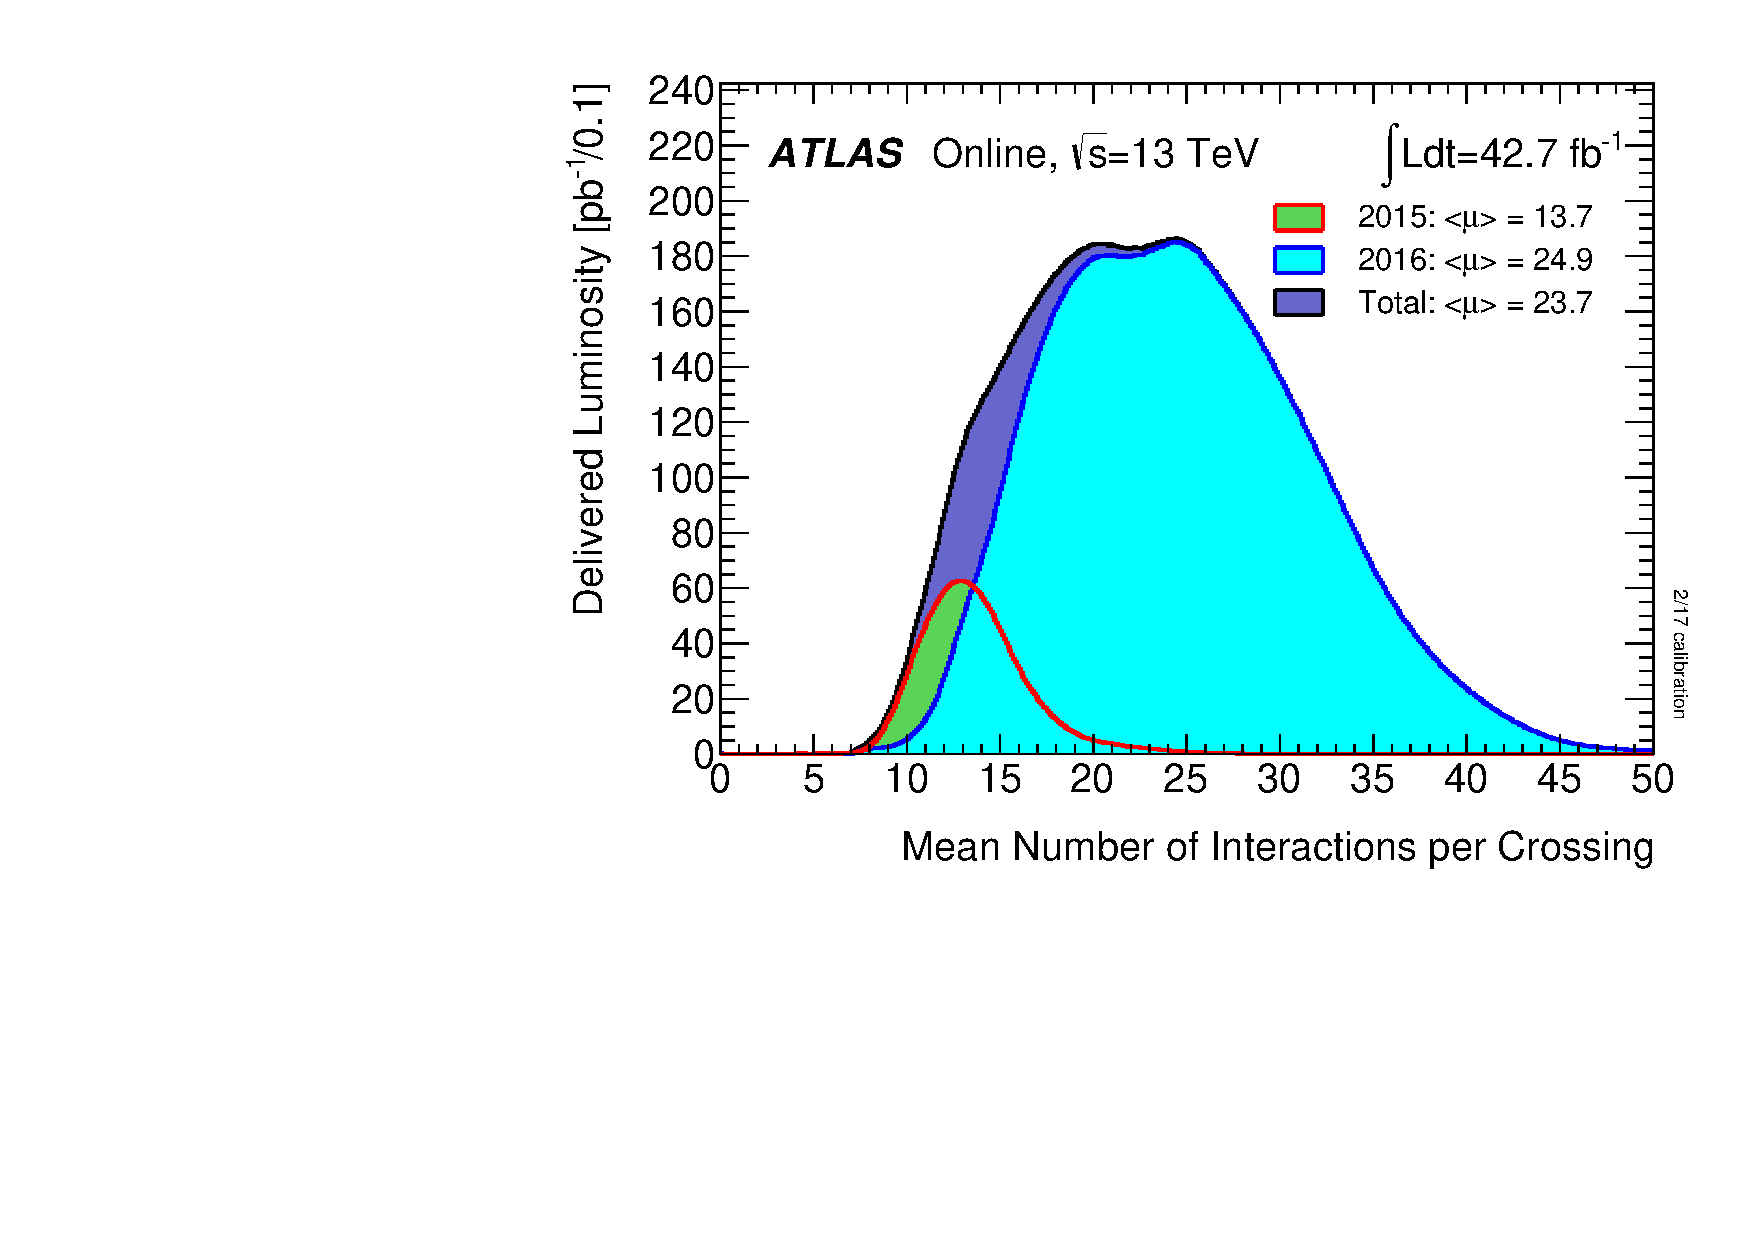
\includegraphics[width=\linewidth]{atlas_lumi_summary}
    \caption{Delivered luminosity as a function of the average number of
      interactions per bunch crossing $\langle \mu \rangle$ during the 2015 and
      2016 data taking periods at $\sqrt{s} = 13$~TeV~\cite{LumiSummaryPlots}.}
    \label{fig:lumi_summary}
\end{figure}
\begin{figure}[!ht]
  \centering
    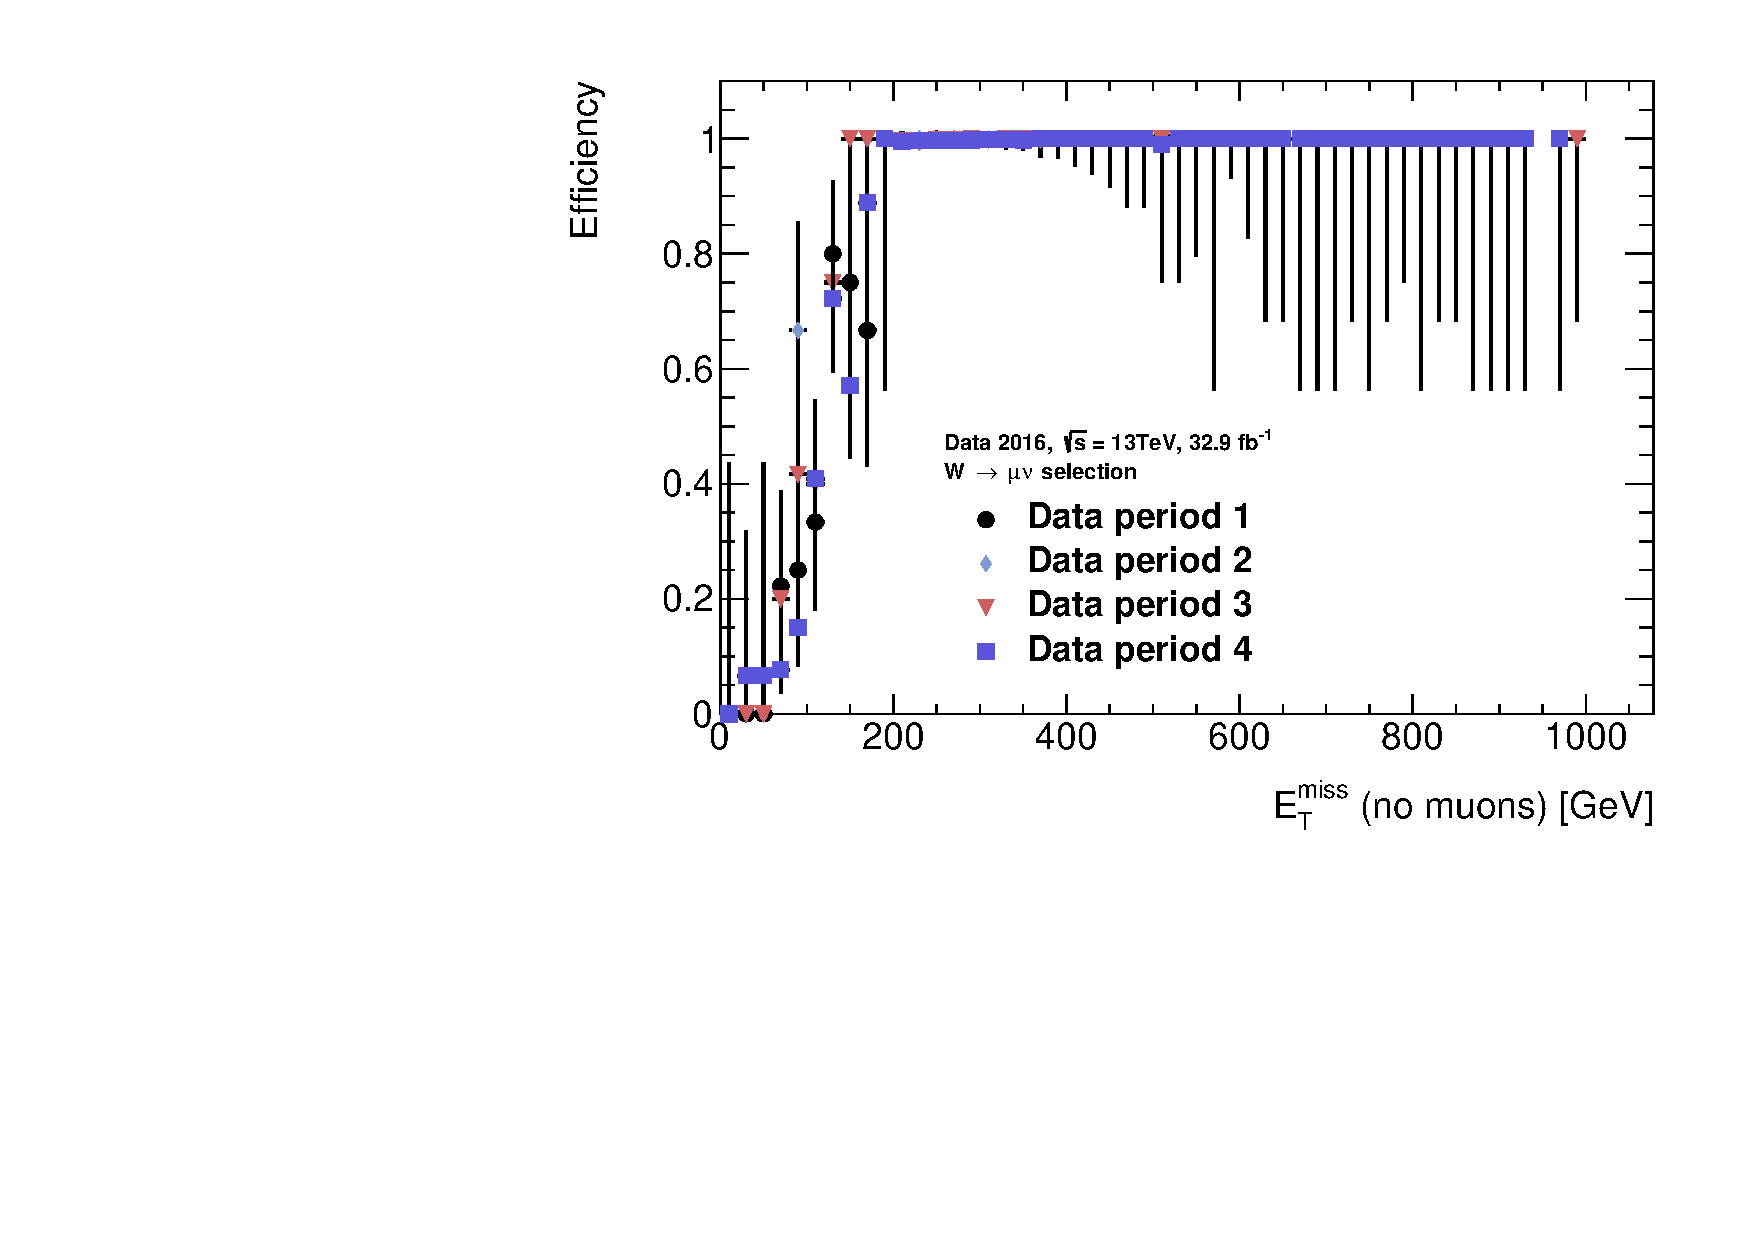
\includegraphics[width=\linewidth]{trigger_efficiency}
    \caption{Trigger efficiency curve as a function of the missing energy for
      the 2016 dataset of 32.9~$\ifb$ estimated in $\wmunuplusjets$ events. The
      four different periods correspond to the run intervals defined in
      \cref{tab:trigger_periods}. The trigger is fully efficient from
      approximately 200~GeV.}
    \label{fig:trigger_efficiency}
\end{figure}
%%% Local Variables:
%%% mode: latex
%%% TeX-master: "../search_for_DM_LED_with_ATLAS"
%%% End:
